\documentclass[margin=10pt]{standalone}
\usepackage{color,xcolor}
\usepackage{makecell}
\usepackage{tikz-qtree, tikz}
\usepackage[utf8]{inputenc}

%%%%%%%%% ANNOTATING IMAGES %%%%%%%%%%%%%
\usepackage{tikz-imagelabels}

\imagelabelset{
   coarse grid color = red,
   fine grid color = gray,
   image label font = \sffamily\bfseries\small,
   image label distance = 2mm,
   image label back = black,
   image label text = white,
   coordinate label font = \sffamily\bfseries\small,
   coordinate label distance = 2mm,
   coordinate label back = none,
   coordinate label text = white,
   annotation font = \normalfont\small,
   arrow distance = 0mm,
   border thickness = 0.6pt,
   arrow thickness = 0.4pt,
   tip size = 1.2mm,
   outer dist = 0.1cm,
}
%%%%%%%%%%%%%%%%%%%%%%%%%%%%%%%%%%%%


\begin{document}
\begin{tikzpicture}
    \node[anchor=south west,inner sep=0] (graph) at (0,0) {
        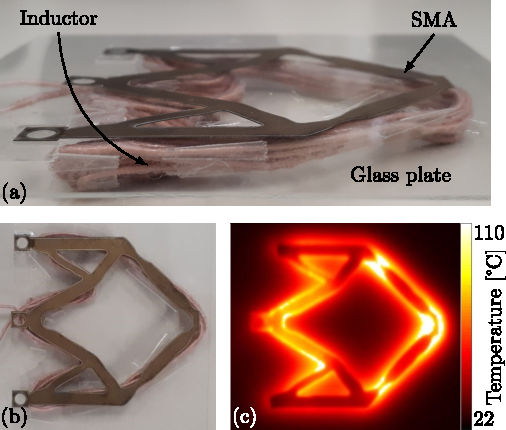
\includegraphics{11_final_results_experiments_heating.pdf}
    };
    \begin{scope}[x={(graph.south east)},y={(graph.north west)}]
        \node [anchor=center, rotate=90] (ylabel) at (1.01,0.25) {\normalsize Temperature [$^\circ$C]};
        \node [anchor=west, rotate=0] at (0.95,-0.005) {\large $22$};
        \node [anchor=west, rotate=0] at (0.95,0.49) {\large $110$};

        \node [anchor=center, rotate=0] at (0.05,0.58) {\large (a)};
        \node [anchor=center, rotate=0] at (0.4,0.04) {\large (b)};
        \node [anchor=center, rotate=0, white] at (0.51,0.04) {\large (c)};
      % \draw[help lines,xstep=.05,ystep=.05] (0,0) grid (1,1);
      %   \foreach \x in {0,1,...,9} { \node [anchor=north] at (\x/10,0) {0.\x}; }
      %   \foreach \y in {0,1,...,9} { \node [anchor=east] at (0,\y/10) {0.\y}; }
    \end{scope}
\end{tikzpicture}
\end{document}
